\documentclass{article}

% =================================================================
% PREAMBLE
% =================================================================
\usepackage{amsmath, amssymb, amsthm} % For math symbols and environments
\usepackage{graphicx}                % For including images
\usepackage[a4paper, margin=1in]{geometry} % For page layout
\usepackage{tikz}                    % For drawing vector graphics
\usepackage{xcolor}                  % For colors
\usepackage{hyperref}                % For hyperlinks
\usepackage{verbatim}                % For simple code blocks

% --- Math Macros ---
\newcommand{\R}{\mathbb{R}}
\newcommand{\D}{\mathcal{D}}
\newcommand{\w}{\mathbf{w}}
\newcommand{\x}{\mathbf{x}}
\newcommand{\y}{\mathbf{y}}
\newcommand{\X}{\mathbf{X}}
\newcommand{\N}{\mathcal{N}}
\newcommand{\E}{\mathbb{E}}
\newcommand{\loss}{\mathcal{L}}
\newcommand{\T}{^\top}

% --- Document Info ---
\title{Lecture 1: An Introduction to Deep Learning}
\author{Recap: Learning and Linear Regression}
\date{}


% =================================================================
% DOCUMENT START
% =================================================================
\begin{document}

\maketitle

\section{The Core Task: Learning from Examples (Supervised Learning)}

At its heart, most of what we'll do is about teaching a computer to learn a function. We start with a dataset of examples, $\D = \{(\x_i, y_i)\}_{i=1}^n$, where each $\x_i$ is an input and $y_i$ is the desired output (or supervision signal). Our goal is to create a flexible function, let's call it $f$, that can learn the relationship between inputs and outputs.

% Figure 8: Dataset Structure (keeping this as is - it's already good)
\begin{figure}[h!]
\centering
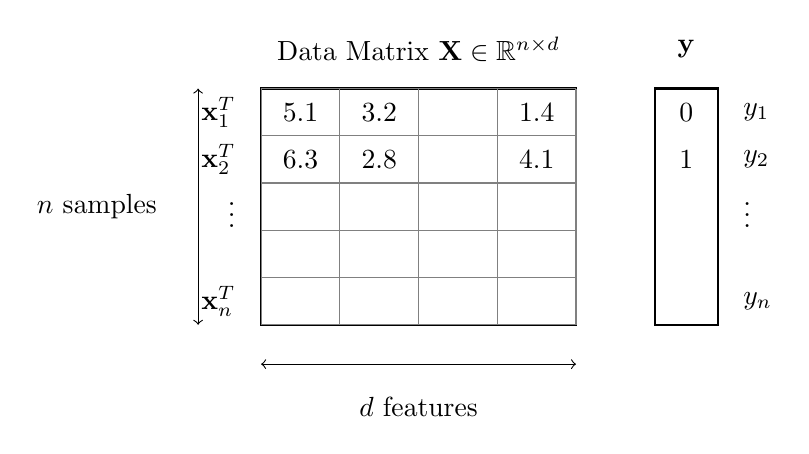
\begin{tikzpicture}[scale=1.0]
  % Dataset matrix X
  \draw[thick] (0,0) rectangle (4,3);
  \node at (2, 3.5) {Data Matrix $\mathbf{X} \in \mathbb{R}^{n \times d}$};
  
  % Grid lines
  \foreach \i in {0,1,2,3,4} {
    \draw[thin, gray] (\i, 0) -- (\i, 3);
  }
  \foreach \i in {0,0.6,1.2,1.8,2.4,3} {
    \draw[thin, gray] (0, \i) -- (4, \i);
  }
  
  % Row labels (samples)
  \node[left] at (-0.2, 2.7) {$\mathbf{x}_1^T$};
  \node[left] at (-0.2, 2.1) {$\mathbf{x}_2^T$};
  \node[left] at (-0.2, 1.5) {$\vdots$};
  \node[left] at (-0.2, 0.3) {$\mathbf{x}_n^T$};
  
  % % Column labels (features)
  % \node[above] at (0.5, 3.2) {$x^{(1)}$};
  % \node[above] at (1.5, 3.2) {$x^{(2)}$};
  % \node[above] at (2.5, 3.2) {$\cdots$};
  % \node[above] at (3.5, 3.2) {$x^{(d)}$};
  
  % Target vector y
  \draw[thick] (5,0) rectangle (5.8,3);
  \node at (5.4, 3.5) {$\mathbf{y}$};
  
  \node[right] at (6, 2.7) {$y_1$};
  \node[right] at (6, 2.1) {$y_2$};
  \node[right] at (6, 1.5) {$\vdots$};
  \node[right] at (6, 0.3) {$y_n$};
  
  % Annotations
  \draw[<->] (-0.8, 0) -- (-0.8, 3);
  \node[left] at (-1.2, 1.5) {$n$ samples};
  
  \draw[<->] (0, -0.5) -- (4, -0.5);
  \node[below] at (2, -0.8) {$d$ features};
  
  % Example values
  \node at (0.5, 2.7) {$5.1$};
  \node at (1.5, 2.7) {$3.2$};
  \node at (3.5, 2.7) {$1.4$};
  \node at (5.4, 2.7) {$0$};
  
  \node at (0.5, 2.1) {$6.3$};
  \node at (1.5, 2.1) {$2.8$};
  \node at (3.5, 2.1) {$4.1$};
  \node at (5.4, 2.1) {$1$};
\end{tikzpicture}
\caption{Dataset structure: Each row represents a sample, each column a feature, and $\mathbf{y}$ contains the target values.}
\end{figure}


\begin{center}
\fcolorbox{black}{gray!10}{
\begin{minipage}{0.9\linewidth}
\centering
\textbf{On the Board: Learning From Examples} \\[1em]
\textbf{Dataset:} $\D=\{(\x_i, y_i)\}_{i=1}^n$, where $\x_i \in \R^d$ and $y_i \in \mathcal{Y}$.

\begin{tabular}{l|l|l}
\textbf{Task} & \textbf{Range of $y$ ($\mathcal{Y}$)} & \textbf{Typical Loss} \\
\hline
Classification & $\{0, \dots, C-1\}$ & Cross-Entropy \\
Regression & $\R$ & Mean-Squared Error \\
Structured Prediction & Images, graphs, sequences & Task-specific
\end{tabular}

\vspace{1em}
We search for $f$ such that
\[ f(\x_i) \approx y_i \quad \text{and the model \textbf{generalises} to unseen data.} \]
\end{minipage}
}
\end{center}

% Figure 7: Improved Types of Learning
\begin{figure}[h!]
\centering
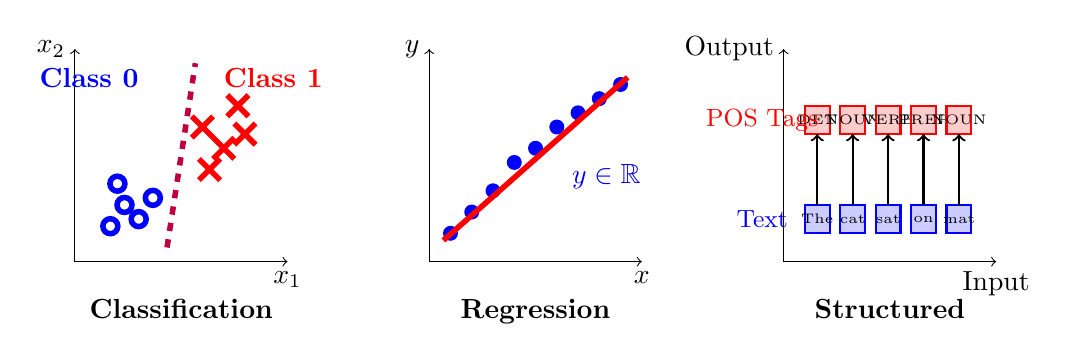
\begin{tikzpicture}[scale=0.9]
  % Classification subplot - improved
  \begin{scope}[xshift=0cm]
    \draw[->] (0,0) -- (3,0) node[below] {$x_1$};
    \draw[->] (0,0) -- (0,3) node[left] {$x_2$};
    
    % Class 1 points (circles) - larger
    \foreach \x/\y in {0.5/0.5, 0.7/0.8, 0.9/0.6, 1.1/0.9, 0.6/1.1} {
      \draw[blue, thick, line width=2pt] (\x, \y) circle (3pt);
    }
    
    % Class 2 points (crosses) - larger
    \foreach \x/\y in {1.8/1.9, 2.1/1.6, 2.3/2.2, 1.9/1.3, 2.4/1.8} {
      \draw[red, thick, line width=2pt] (\x-0.15, \y-0.15) -- (\x+0.15, \y+0.15);
      \draw[red, thick, line width=2pt] (\x-0.15, \y+0.15) -- (\x+0.15, \y-0.15);
    }
    
    % Decision boundary
    \draw[thick, purple, dashed, line width=2pt] (1.3, 0.2) -- (1.7, 2.8);
    
    \node[below] at (1.5, -0.4) {\textbf{Classification}};
    \node[blue] at (0.2, 2.6) {\textbf{Class 0}};
    \node[red] at (2.8, 2.6) {\textbf{Class 1}};
  \end{scope}
  
  % Regression subplot - improved
  \begin{scope}[xshift=5cm]
    \draw[->] (0,0) -- (3,0) node[below] {$x$};
    \draw[->] (0,0) -- (0,3) node[left] {$y$};
    
    % Continuous data points - larger
    \foreach \x/\y in {0.3/0.4, 0.6/0.7, 0.9/1.0, 1.2/1.4, 1.5/1.6, 1.8/1.9, 2.1/2.1, 2.4/2.3, 2.7/2.5} {
      \fill[blue] (\x, \y) circle (3pt);
    }
    
    % Regression line - thicker
    \draw[thick, red, line width=2pt] (0.2, 0.3) -- (2.8, 2.6);
    
    \node[below] at (1.5, -0.4) {\textbf{Regression}};
    \node[blue] at (2.5, 1.2) {$y \in \mathbb{R}$};
  \end{scope}
  
  % Structured prediction - much improved
  \begin{scope}[xshift=10cm]
    \draw[->] (0,0) -- (3,0) node[below] {Input};
    \draw[->] (0,0) -- (0,3) node[left] {Output};
    
    % Better sequence visualization
    \foreach \i/\word in {0.3/The, 0.8/cat, 1.3/sat, 1.8/on, 2.3/mat} {
      \draw[thick, blue, fill=blue!20] (\i, 0.4) rectangle +(0.35, 0.4);
      \node[font=\tiny] at (\i+0.175, 0.6) {\word};
    }
    
    \foreach \i/\tag in {0.3/DET, 0.8/NOUN, 1.3/VERB, 1.8/PREP, 2.3/NOUN} {
      \draw[thick, red, fill=red!20] (\i, 1.8) rectangle +(0.35, 0.4);
      \node[font=\tiny] at (\i+0.175, 2.0) {\tag};
    }
    
    % Arrows showing mapping
    \foreach \i in {0.475, 0.975, 1.475, 1.975, 2.475} {
      \draw[thick, ->] (\i, 0.8) -- (\i, 1.8);
    }
    
    \node[below] at (1.5, -0.4) {\textbf{Structured}};
    \node[blue, font=\small] at (-0.3, 0.6) {Text};
    \node[red, font=\small] at (-0.3, 2.0) {POS Tags};
  \end{scope}
\end{tikzpicture}
\caption{Three main types of supervised learning: Classification (discrete labels), Regression (continuous values), and Structured Prediction (complex outputs like sequences).}
\end{figure}




\section{Why is Learning Hard? The Challenge of Generalization}

This task sounds simple, but it's fundamentally hard. For any finite set of examples, there are infinitely many functions that fit them perfectly. To make progress, our learning algorithm needs a ``nudge'' in the right direction. This guiding assumption is called its \textbf{inductive bias}.

\begin{itemize}
    \item A \textbf{linear model} has a \textbf{strong bias} (it assumes the world is linear). It's simple but often fails on complex data (low variance, high bias).
    \item A \textbf{deep neural network} has a \textbf{weak bias}. Its flexibility lets it learn complex patterns but risks \textbf{overfitting}---memorizing the training data instead of the underlying rule (high variance, low bias).
\end{itemize}

We search for parameters $\hat{\w}$ of a model family $f_\w$ such that
\[ f_{\hat{\w}}(\x_i) \approx y_i \quad \text{and the model \textbf{generalises} to unseen data.} \]

The key to modern deep learning is to use a flexible model and combat overfitting with massive amounts of data and regularization.


% Figure 5: Improved Model Complexity Comparison
\begin{figure}[h!]
\centering
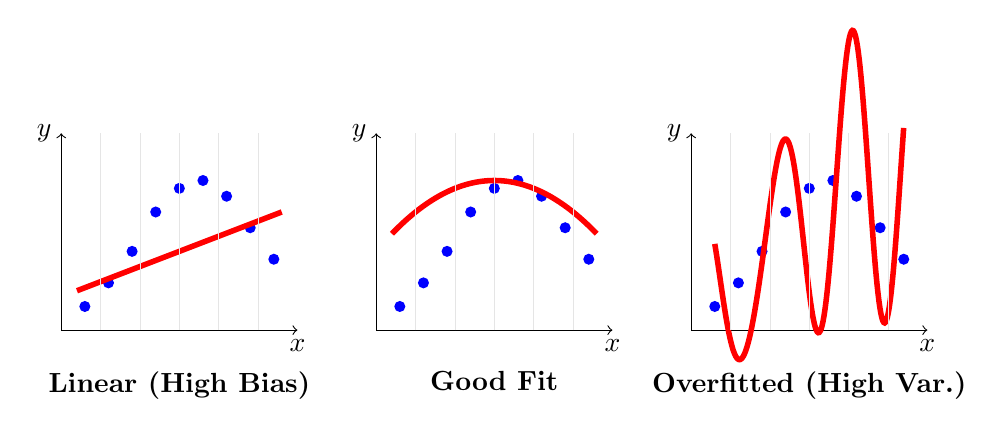
\begin{tikzpicture}[scale=1.0]
  % Subplot 1: Linear (Underfitting) - improved
  \begin{scope}[xshift=0cm]
    \draw[->] (0,0) -- (3,0) node[below] {$x$};
    \draw[->] (0,0) -- (0,2.5) node[left] {$y$};
    
    % More realistic non-linear data
    \foreach \x/\y in {0.3/0.3, 0.6/0.6, 0.9/1.0, 1.2/1.5, 1.5/1.8, 1.8/1.9, 2.1/1.7, 2.4/1.3, 2.7/0.9} {
      \fill[blue] (\x, \y) circle (2pt);
    }
    
    % Linear fit - clearly inadequate
    \draw[thick, red, line width=2pt] (0.2, 0.5) -- (2.8, 1.5);
    \node[below] at (1.5, -0.4) {\textbf{Linear (High Bias)}};
    
    % Grid
    \foreach \x in {0.5,1,1.5,2,2.5} {
      \draw[very thin, gray!20] (\x, 0) -- (\x, 2.5);
    }
  \end{scope}
  
  % Subplot 2: Good fit - improved
  \begin{scope}[xshift=4cm]
    \draw[->] (0,0) -- (3,0) node[below] {$x$};
    \draw[->] (0,0) -- (0,2.5) node[left] {$y$};
    
    % Same data points
    \foreach \x/\y in {0.3/0.3, 0.6/0.6, 0.9/1.0, 1.2/1.5, 1.5/1.8, 1.8/1.9, 2.1/1.7, 2.4/1.3, 2.7/0.9} {
      \fill[blue] (\x, \y) circle (2pt);
    }
    
    % Better polynomial fit
    \draw[thick, red, line width=2pt, domain=0.2:2.8, samples=100] plot (\x, {-0.4*(\x-1.5)^2 + 1.9});
    \node[below] at (1.5, -0.4) {\textbf{Good Fit}};
    
    % Grid
    \foreach \x in {0.5,1,1.5,2,2.5} {
      \draw[very thin, gray!20] (\x, 0) -- (\x, 2.5);
    }
  \end{scope}
  
  % Subplot 3: Overfitted - more realistic
  \begin{scope}[xshift=8cm]
    \draw[->] (0,0) -- (3,0) node[below] {$x$};
    \draw[->] (0,0) -- (0,2.5) node[left] {$y$};
    
    % Same data points
    \foreach \x/\y in {0.3/0.3, 0.6/0.6, 0.9/1.0, 1.2/1.5, 1.5/1.8, 1.8/1.9, 2.1/1.7, 2.4/1.3, 2.7/0.9} {
      \fill[blue] (\x, \y) circle (2pt);
    }
    
    % More realistic overfitted curve
    \draw[thick, red, line width=2pt, domain=0.3:2.7, samples=200] 
      plot (\x, {0.3 + 0.8*\x + 1.5*sin(7*\x r) + 0.5*cos(9*\x r) - 0.2*(\x-1.5)^2});
    \node[below] at (1.5, -0.4) {\textbf{Overfitted (High Var.)}};
    
    % Grid
    \foreach \x in {0.5,1,1.5,2,2.5} {
      \draw[very thin, gray!20] (\x, 0) -- (\x, 2.5);
    }
  \end{scope}
\end{tikzpicture}
\caption{Model Complexity: From left to right - underfitting (high bias), good fit, overfitting (high variance).}
\end{figure}


\section{Linear Regression: A Foundational Recap}

% Figure 3: Improved Linear Regression
\begin{figure}[h!]
\centering
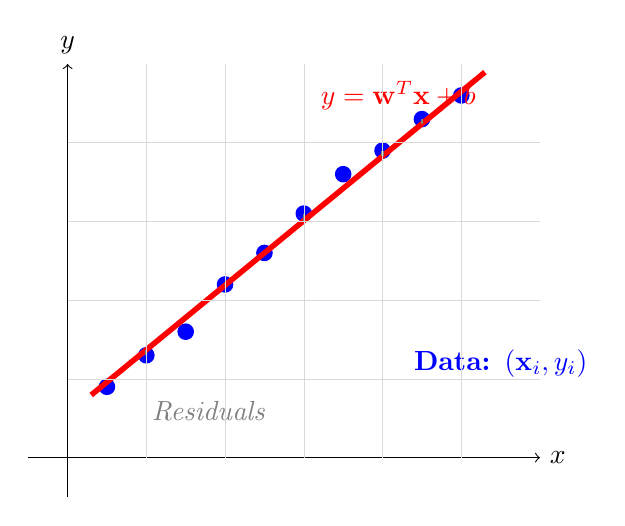
\begin{tikzpicture}[scale=1.0]
  \draw[->] (-0.5,0) -- (6,0) node[right] {$x$};
  \draw[->] (0,-0.5) -- (0,5) node[above] {$y$};
  
  % More realistic data points with slight scatter
  \foreach \x/\y in {0.5/0.9, 1/1.3, 1.5/1.6, 2/2.2, 2.5/2.6, 3/3.1, 3.5/3.6, 4/3.9, 4.5/4.3, 5/4.6} {
    \fill[blue] (\x, \y) circle (3pt);
  }
  
  % Regression line - thicker
  \draw[thick, red, line width=2pt, domain=0.3:5.3] plot (\x, {0.82*\x + 0.55});
  \node[red] at (4.2, 4.6) {$y = \mathbf{w}^T\mathbf{x} + b$};
  
  % More visible residuals
  \draw[dashed, gray, thick] (1, 1.3) -- (1, 1.37);
  \draw[dashed, gray, thick] (2, 2.2) -- (2, 2.19);
  \draw[dashed, gray, thick] (3, 3.1) -- (3, 3.01);
  \draw[dashed, gray, thick] (4, 3.9) -- (4, 3.83);
  \draw[dashed, gray, thick] (4.5, 4.3) -- (4.5, 4.24);
  
  % Better labels
  \node[blue] at (5.5, 1.2) {\textbf{Data: $(\mathbf{x}_i, y_i)$}};
  \node[gray] at (1.8, 0.6) {\textit{Residuals}};
  
  % Grid for better readability
  \foreach \x in {1,2,3,4,5} {
    \draw[very thin, gray!30] (\x, 0) -- (\x, 5);
  }
  \foreach \y in {1,2,3,4} {
    \draw[very thin, gray!30] (0, \y) -- (6, \y);
  }
\end{tikzpicture}
\caption{Linear Regression: Finding the best line through the data points by minimizing squared residuals.}
\end{figure}
Let's solidify these concepts with linear regression. It's a perfect microcosm of the entire supervised learning process.

\subsection{Model \& Geometry}

We assume a linear relationship: $y = \w\T\x + b$. Geometrically, the weight vector $\w$ defines the orientation (slope) of a hyperplane, and the bias $b$ shifts it.

\begin{center}
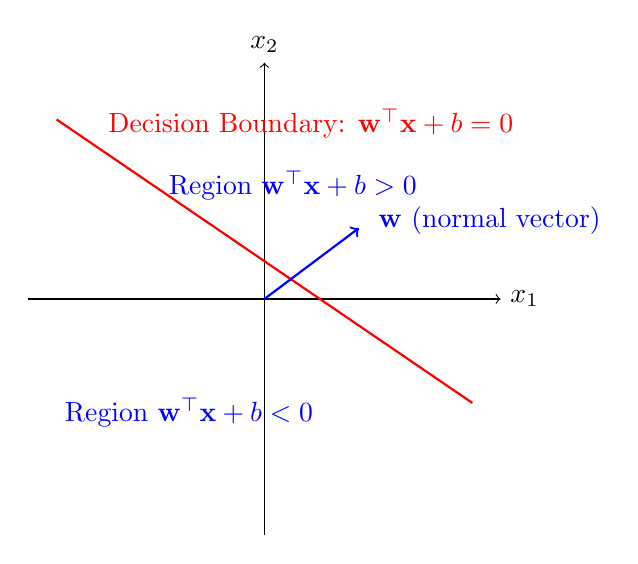
\begin{tikzpicture}[scale=1.2]
  \draw[->] (-2.5,0)--(2.5,0) node[right] {$x_1$};
  \draw[->] (0,-2.5)--(0,2.5) node[above] {$x_2$};
  \draw[thick, red] (-2.2, 1.9) -- (2.2, -1.1) node[pos=0.1, above right] {Decision Boundary: $\w\T\x + b = 0$};
  \draw[blue, thick, ->] (0,0) -- (1, 0.75) node[pos=1.1, right] {$\w$ (normal vector)};
  \node[blue] at (0.3, 1.2) {Region $\w\T\x+b > 0$};
  \node[blue] at (-0.8, -1.2) {Region $\w\T\x+b < 0$};
\end{tikzpicture}
\end{center}

\subsection{The Least-Squares Loss Function}

To find the ``best'' hyperplane, we need to quantify error. The standard choice is the \textbf{Mean Squared Error (MSE)}, which we aim to minimize.
\begin{equation}
    \loss(\w, b) = \frac{1}{n} \sum_{i=1}^n (y_i - (\w\T\x_i + b))^2
\end{equation}
By augmenting our data matrix $\X \in \R^{n \times d}$ with a column of ones and our weight vector $\w \in \R^d$ with the bias term $b$, we can write this compactly. Let $\X_{aug} \in \R^{n \times (d+1)}$ and $\w_{aug} \in \R^{d+1}$.
\begin{equation}
    \loss(\w) = \frac{1}{n} \|\y - \X\w\|_2^2
\end{equation}

\subsection{Optimization: Finding the Best Parameters}

\paragraph{Method 1: The Analytical Solution.} For this specific problem, we can find the exact minimizer by setting the gradient $\nabla_\w \loss(\w) = 0$. This yields the \textbf{Normal Equations}:
\begin{equation}
    \hat{\w}_{\text{OLS}} = (\X\T\X)^{-1}\X\T\y
\end{equation}
This is elegant, but rarely used in deep learning due to the computational cost ($O(d^3)$) and non-existence of such solutions for more complex models.

\paragraph{Method 2: Gradient Descent.} The workhorse of deep learning. We start with a random guess for $\w$ and iteratively take small steps in the direction of the negative gradient.
\begin{equation}
    \w^{(t+1)} = \w^{(t)} - \eta \nabla_\w \loss(\w^{(t)})
\end{equation}
For the MSE loss, the gradient is $\nabla_\w \loss(\w) = \frac{2}{n}\X\T(\X\w - \y)$. This gives the update rule:
\begin{equation}
    \w^{(t+1)} = \w^{(t)} - \eta \frac{2}{n}\X\T(\X\w^{(t)} - \y)
\end{equation}
This iterative process is exactly what modern deep learning frameworks automate.


% Figure 9: Improved Normal Equations Geometry
\begin{figure}[h!]
\centering
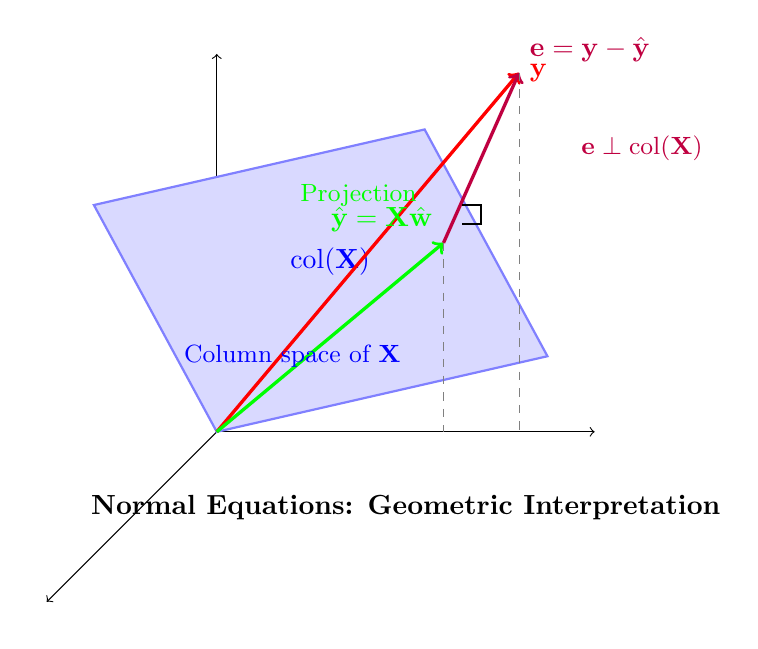
\begin{tikzpicture}[scale=1.2]
  % 3D-like coordinate system
  \draw[->] (0,0) -- (4,0) node[right] {};
  \draw[->] (0,0) -- (0,4) node[above] {};
  \draw[->] (0,0) -- (-1.8,-1.8) node[below left] {};
  
  % Column space (more 3D-like plane)
  \fill[blue!15] (0,0) -- (3.5,0.8) -- (2.2,3.2) -- (-1.3,2.4) -- cycle;
  \draw[thick, blue!50] (0,0) -- (3.5,0.8) -- (2.2,3.2) -- (-1.3,2.4) -- cycle;
  \node[blue] at (1.2, 1.8) {$\text{col}(\mathbf{X})$};
  
  % Target vector y (outside column space) - more prominent
  \draw[very thick, red, ->] (0,0) -- (3.2,3.8) node[right] {$\mathbf{y}$};
  
  % Projection onto column space - more prominent
  \draw[very thick, green, ->] (0,0) -- (2.4,2.0) node[above left] {$\hat{\mathbf{y}} = \mathbf{X}\hat{\mathbf{w}}$};
  
  % Residual vector (orthogonal) - more prominent
  \draw[very thick, purple, ->] (2.4,2.0) -- (3.2,3.8) node[above right] {$\mathbf{e} = \mathbf{y} - \hat{\mathbf{y}}$};
  
  % Clearer orthogonality symbol
  \draw[thick] (2.6, 2.2) -- (2.8, 2.2) -- (2.8, 2.4) -- (2.6, 2.4);
  
  % Additional annotations
  \draw[dashed, gray] (2.4, 2.0) -- (2.4, 0);
  \draw[dashed, gray] (3.2, 3.8) -- (3.2, 0);
  
  % Labels
  \node at (2, -0.8) {\textbf{Normal Equations: Geometric Interpretation}};
  \node[blue, font=\small] at (0.8, 0.8) {Column space of $\mathbf{X}$};
  \node[purple, font=\small] at (4.5, 3.0) {$\mathbf{e} \perp \text{col}(\mathbf{X})$};
  \node[green, font=\small] at (1.5, 2.5) {Projection};
\end{tikzpicture}
\caption{Normal Equations Geometry: The optimal solution projects $\mathbf{y}$ onto the column space of $\mathbf{X}$. The residual is orthogonal to the column space.}
\end{figure}


\newpage
% -----------------------------------------------------------------
\subsection{The Bias-Variance Trade-Off}
% -----------------------------------------------------------------
Our learned weights, $\hat{\w}$, are a function of the training data $\D$. Since $\D$ is a random sample, $\hat{\w}$ is a random variable. 
A model’s \emph{expected generalisation error} on a new point can be decomposed:
\begin{equation}\label{eq:bv_decomp}
\operatorname{Err}(\hat f)=\E_{(\x,y)\sim p_{\text{data}}}\!\bigl[(y-\hat f(\x))^{2}\bigr]=
\E\!\bigl[(\hat y-y)^2\bigr]
    =\underbrace{\bigl(\E[\hat y]-y\bigr)^{2}}_{\text{Bias}^{2}}
     +\underbrace{\E\!\bigl[(\hat y-\E[\hat y])^{2}\bigr]}_{\text{Variance}}
     +\underbrace{\sigma_{\varepsilon}^{2}}_{\text{Irreducible noise}},
\end{equation}


\begin{itemize}
\item \textbf{Bias} measures how far the \emph{average} model prediction deviates
      from the truth because of limiting assumptions (e.g.\ linearity). A simple model on complex data is systematically wrong (underfitting).
\item \textbf{Variance} measures how much the prediction would change if we
      collected a fresh training set—i.e.\ the model’s sensitivity to sampling
      noise. Error from sensitivity to small fluctuations in the training set. A complex model can fit the noise (overfitting).
\item \textbf{Irreducible noise} captures randomness inherent to the data
      generating process and cannot be learned away.
\end{itemize}

\paragraph{Key take-aways (without the polemics).}
\begin{enumerate}
\item \textbf{Bias and variance are \emph{orthogonal} concepts, not a see-saw.}  
      Increases in model capacity \emph{can} reduce bias \emph{without} forcing
      variance to sky-rocket if accompanied by
      \begin{itemize}
        \item more data,
        \item suitable regularisation (e.g.\ weight decay, early stopping),
        \item inductive biases matched to the task.
      \end{itemize}
      The classical ``U-shaped'' textbook diagram is therefore a helpful cartoon,
      not a law of nature.\footnote{See B.~Neal, \emph{“On the Bias–Variance
      Trade-Off: Textbooks Need an Update”}, 2020, for a lucid, data-driven
      exposition.}%
      % :contentReference[oaicite:0]{index=0}
\item \textbf{Regularisation tactics.}
      Adding an $L_{2}$ penalty (\emph{Ridge}) gently increases bias while
      often slashing variance, delivering a net gain in generalisation.
      Other forms (dropout, data augmentation, ensembling) act similarly:
      they nudge the learning dynamics toward parameters that behave
      consistently across possible datasets.
\item \textbf{Sample size matters.}
      For a fixed hypothesis class, variance decays as $O\!\bigl(1/n\bigr)$,
      whereas bias is controlled by the model family.  Collecting more data
      is the most principled antidote to high variance.
\item \textbf{Deep-learning perspective.}
      Modern over-parameterised networks may operate in a ``sweet-spot'' regime
      where implicit regularisation (stochastic gradient descent, architectural
      constraints) keeps variance in check even though capacity is enormous.
      We postpone the finer points to the discussion session; for now, the
      bias–variance lens still provides a first-order mental model.
\end{enumerate}

\vspace{0.5em}
\noindent
\textit{Practical moral:} strive to balance simplicity (lower bias) with
stability (lower variance) using \emph{both} model design and data/algorithm
levers—regularisation, larger datasets, and task-appropriate inductive bias.

% Figure 1: Improved Bias-Variance Tradeoff
\begin{figure}[h!]
\centering
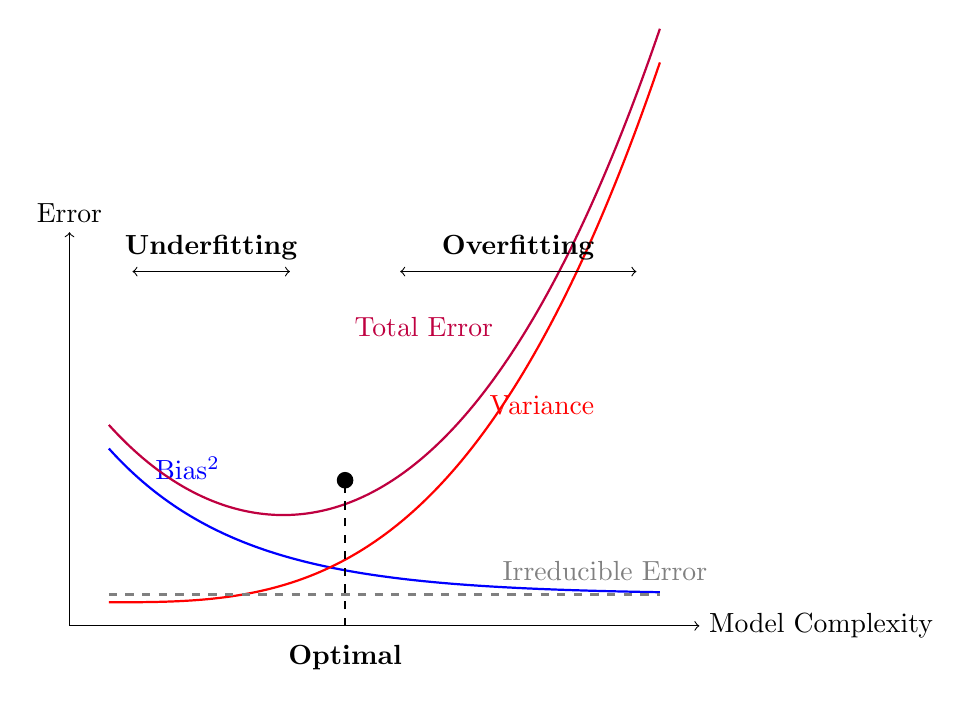
\begin{tikzpicture}[scale=1.0]
  \draw[->] (0,0) -- (8,0) node[right] {Model Complexity};
  \draw[->] (0,0) -- (0,5) node[above] {Error};
  
  % Bias curve (smoother decreasing)
  \draw[thick, blue, domain=0.5:7.5, samples=150] plot (\x, {2.5*exp(-0.6*\x) + 0.4});
  \node[blue] at (1.5, 2.0) {Bias$^2$};
  
  % Variance curve (smoother increasing)
  \draw[thick, red, domain=0.5:7.5, samples=150] plot (\x, {0.02*(\x-0.5)^3 + 0.3});
  \node[red] at (6, 2.8) {Variance};
  
  % Total error curve (smoother U-shape)
  \draw[thick, purple, domain=0.5:7.5, samples=150] plot (\x, {2.5*exp(-0.6*\x) + 0.02*(\x-0.5)^3 + 0.7});
  \node[purple] at (4.5, 3.8) {Total Error};
  
  % Irreducible error line
  \draw[thick, gray, dashed] (0.5, 0.4) -- (7.5, 0.4);
  \node[gray] at (6.8, 0.7) {Irreducible Error};
  
  % Optimal point - more prominent
  \coordinate (opt) at (3.5, 1.85);
  \draw[thick, black, dashed] (3.5, 0) -- (opt);
  \fill[black] (opt) circle (3pt);
  \node[black] at (3.5, -0.4) {\textbf{Optimal}};
  
  % Region labels with arrows
  \draw[<->] (0.8, 4.5) -- (2.8, 4.5);
  \node at (1.8, 4.8) {\textbf{Underfitting}};
  \draw[<->] (4.2, 4.5) -- (7.2, 4.5);
  \node at (5.7, 4.8) {\textbf{Overfitting}};
\end{tikzpicture}
\caption{Bias-Variance Tradeoff: As model complexity increases, bias decreases but variance increases. The optimal point minimizes total error.}
\end{figure}

% Figure 2: Improved Training vs Validation Error Curves
\begin{figure}[h!]
\centering
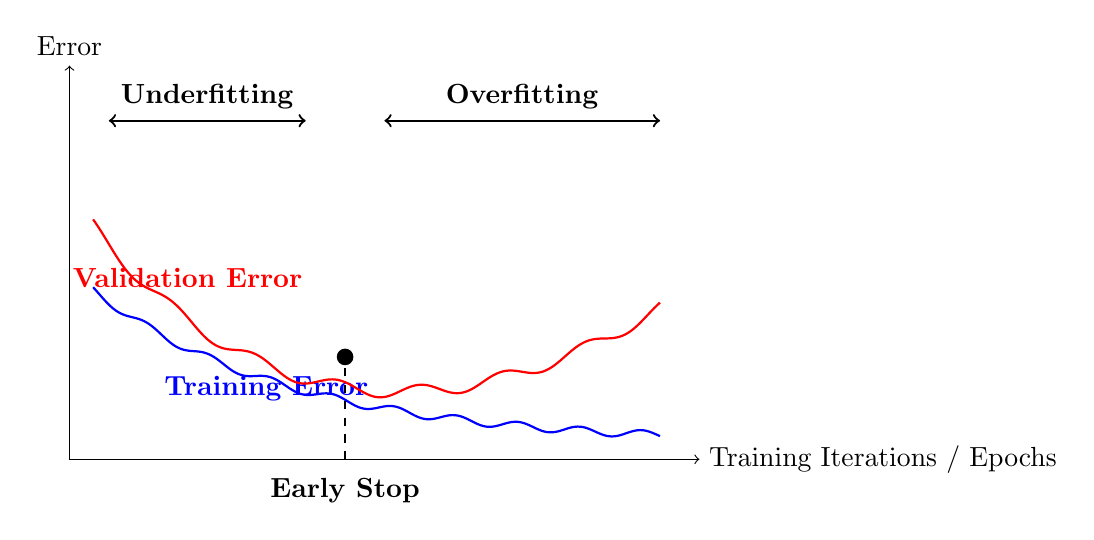
\begin{tikzpicture}[scale=1.0]
  \draw[->] (0,0) -- (8,0) node[right] {Training Iterations / Epochs};
  \draw[->] (0,0) -- (0,5) node[above] {Error};
  
  % Training error (smooth decreasing with realistic noise)
  \draw[thick, blue, domain=0.3:7.5, samples=200] plot (\x, {2.2*exp(-0.4*\x) + 0.2 + 0.05*sin(8*\x r)});
  \node[blue] at (2.5, 0.9) {\textbf{Training Error}};
  
  % Validation error (realistic U-shaped with noise)
  \draw[thick, red, domain=0.3:7.5, samples=200] plot (\x, {1.8*exp(-0.5*\x) + 0.08*(\x-3.5)^2 + 0.6 + 0.08*sin(6*\x r)});
  \node[red] at (1.5, 2.3) {\textbf{Validation Error}};
  
  % Early stopping point - more prominent
  \coordinate (stop) at (3.5, 1.3);
  \draw[thick, black, dashed] (3.5, 0) -- (stop);
  \fill[black] (stop) circle (3pt);
  \node[black] at (3.5, -0.4) {\textbf{Early Stop}};
  
  % Clear region separation
  \draw[<->, thick] (0.5, 4.3) -- (3, 4.3);
  \node at (1.75, 4.6) {\textbf{Underfitting}};
  \draw[<->, thick] (4, 4.3) -- (7.5, 4.3);
  \node at (5.75, 4.6) {\textbf{Overfitting}};
\end{tikzpicture}
\caption{Training vs Validation Error: The validation error starts increasing when overfitting begins. Early stopping prevents overfitting.}
\end{figure}

\subsection{Combating Overfitting with Regularization}
To control high variance, we can add a penalty for model complexity to the loss function. \textbf{Ridge Regression} uses an $L_2$ penalty on the weights:
\begin{equation}
    \loss_\lambda(\w) = \frac{1}{n}\|\y - \X\w\|_2^2 + \lambda\|\w\|_2^2
\end{equation}
This biases the model towards solutions with smaller weights, which are often simpler and generalize better. This changes the closed-form solution to:
\begin{equation}
    \hat{\w}_{\text{ridge}} = (\X\T\X + \lambda I)^{-1}\X\T\y
\end{equation}
Adding regularization tends to increase bias slightly while significantly decreasing variance.

\subsection{A Probabilistic View: Maximum Likelihood Estimation (MLE)}
The MSE loss is not arbitrary. Assume that our data is generated by a linear process with Gaussian noise: $y = \w\T\x + b + \epsilon$, where $\epsilon \sim \N(0, \sigma^2)$. This implies the conditional probability:
\begin{equation}
    p(y | \x; \w, b) = \N(y | \w\T\x + b, \sigma^2)
\end{equation}
The goal of MLE is to find parameters that maximize the log-likelihood of the data:
\begin{align*}
    \log \mathcal{L}(\w, b) &= \sum_{i=1}^n \log p(y_i | \x_i; \w, b) \\
    &= \sum_{i=1}^n \log \left( \frac{1}{\sqrt{2\pi\sigma^2}} \exp\left(-\frac{(y_i - (\w\T\x_i+b))^2}{2\sigma^2}\right) \right) \\
    &= C - \frac{1}{2\sigma^2} \sum_{i=1}^n (y_i - (\w\T\x_i+b))^2
\end{align*}
Maximizing this expression is equivalent to \textbf{minimizing the sum of squared errors}.




\subsection{Regularization in High Dimensions: Ridge vs. Lasso}

While the previous simulation showed the basic bias-variance trade-off, the true power of regularization shines in high-dimensional settings where many features might be irrelevant. To demonstrate this, we introduce another powerful technique: \textbf{Lasso Regression}.

\paragraph{Lasso ($L_1$ Regularization)}
Lasso (Least Absolute Shrinkage and Selection Operator) is similar to Ridge, but it uses the $L_1$ norm of the weights as its penalty term.
\begin{equation}
    \loss_\lambda(\w) = \frac{1}{n}\|\y - \X\w\|_2^2 + \lambda\|\w\|_1 = \frac{1}{n}\|\y - \X\w\|_2^2 + \lambda \sum_{j=1}^d |w_j|
\end{equation}
This seemingly small change from $\|\w\|_2^2$ to $\|\w\|_1$ has a profound effect. The $L_1$ penalty encourages \textbf{sparsity}, meaning it forces the coefficients of the least informative features to become \textit{exactly zero}. Therefore, Lasso doesn't just shrink coefficients; it performs automatic \textbf{feature selection}, making it invaluable when you suspect many of your features are noise.


% Figure 6: Improved Regularization Effect
\begin{figure}[h!]
\centering
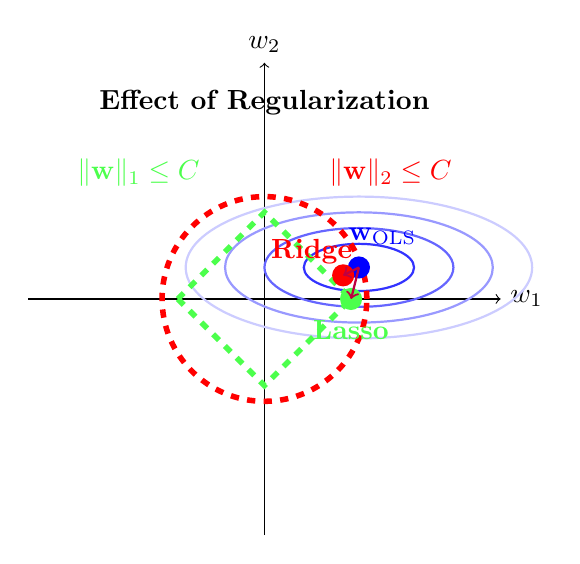
\begin{tikzpicture}[scale=1.0]
  \draw[->] (-3,0) -- (3,0) node[right] {$w_1$};
  \draw[->] (0,-3) -- (0,3) node[above] {$w_2$};
  
  % Loss contours (more elongated to show effect better)
  \draw[thick, blue!20] (1.2,0.4) ellipse (2.2 and 0.9);
  \draw[thick, blue!40] (1.2,0.4) ellipse (1.7 and 0.7);
  \draw[thick, blue!60] (1.2,0.4) ellipse (1.2 and 0.5);
  \draw[thick, blue!80] (1.2,0.4) ellipse (0.7 and 0.3);
  
  % L2 constraint (circle) - more prominent
  \draw[thick, red, dashed, line width=2pt] (0,0) circle (1.3);
  \node[red] at (1.6, 1.6) {$\|\mathbf{w}\|_2 \leq C$};
  
  % L1 constraint (diamond) - more prominent
  \draw[thick, green!70, dashed, line width=2pt] (-1.1,0) -- (0,1.1) -- (1.1,0) -- (0,-1.1) -- cycle;
  \node[green!70] at (-1.6, 1.6) {$\|\mathbf{w}\|_1 \leq C$};
  
  % Points - larger and more prominent
  \fill[blue] (1.2, 0.4) circle (4pt);
  \node[blue] at (1.5, 0.8) {$\mathbf{w}_{\text{OLS}}$};
  
  \fill[red] (1.0, 0.3) circle (4pt);
  \node[red] at (0.6, 0.6) {\textbf{Ridge}};
  
  \fill[green!70] (1.1, 0) circle (4pt);
  \node[green!70] at (1.1, -0.4) {\textbf{Lasso}};
  
  % Title
  \node at (0, 2.5) {\textbf{Effect of Regularization}};
  
  % Arrows showing the effect
  \draw[purple, thick, ->] (1.2, 0.4) -- (1.0, 0.3);
  \draw[purple, thick, ->] (1.2, 0.4) -- (1.1, 0);
\end{tikzpicture}
\caption{Regularization: L2 (Ridge) shrinks weights uniformly, L1 (Lasso) can set weights to zero for sparsity.}
\end{figure}


\paragraph{The Experiment}
In the accompanying Python file, \texttt{lecture1\_regularization\_comparison.py}, we set up a more challenging problem:
\begin{enumerate}
    \item We create a high-dimensional dataset with 20 features ($d=20$).
    \item Critically, only the first 5 of these features are actually used to generate the output $y$. The other 15 are pure noise.
    \item We then train three models on this data: standard OLS, Ridge, and Lasso.
\end{enumerate}
Our goal is to see how well each model can recover the ``true'' weights, which should be non-zero for the first 5 features and zero for the rest. We evaluate the models based on two metrics:
\begin{itemize}
    \item \textbf{Weight MSE}: The mean squared error between the model's estimated weights and the true weights. A lower value means the model's parameters are closer to reality.
    \item \textbf{Sparsity}: The number of weights the model sets to (near) zero. The ideal model would set the 15 irrelevant feature weights to zero.
\end{itemize}

\paragraph{Interpreting the Results}
The script's output clearly demonstrates the strengths of each method:
\begin{itemize}
    \item \textbf{OLS} has a very high Weight MSE. It completely overfits to the 15 noisy features, assigning them large, incorrect weights. It finds no zero-weight features.
    \item \textbf{Ridge Regression} does much better. Its $L_2$ penalty shrinks the irrelevant weights towards zero, significantly reducing the overall error. However, it does not set them \textit{exactly} to zero.
    \item \textbf{Lasso Regression} performs the best in this scenario. It also reduces the overall error, but most importantly, it correctly identifies the noisy features and sets their corresponding weights to zero. This results in a sparse, more interpretable model that has effectively performed feature selection.
\end{itemize}
This simulation provides a practical look at why regularization is not just a theoretical concept, but an essential tool for building robust machine learning models in the face of high-dimensional, noisy data.






\section{Bridging to the Next Lecture}
The concepts from linear regression are not just an analogy; they are the literal foundation of deep networks. A single neuron in a neural network performs a very similar computation.
\[ \underbrace{y = \w\T\x + b}_{\text{Today: Linear Regression}} \quad \xrightarrow{\text{Add a non-linearity}} \quad \underbrace{y = \sigma(\w\T\x + b)}_{\text{Next: A Perceptron / Neuron}} \]
Training these complex networks still relies on minimizing a loss function with gradient descent. The core concepts of capacity, over/under-fitting, bias-variance, and regularization will reappear constantly.

\newpage





\end{document}